\subsection{Tuning methods}
With a view to ensure a tracking communication between the drone and its ground station, and thus, keep a proper angle of the directions of the antennas, a controller has been designed.\par

The actuator to be controlled is a servomotor having the desired characteristics for this application.  Reaching speed, accuracy and weight of the antenna were taken into account to determine the appropriate motor. Based on the above mentioned, different controllers were tested as a PID, PI, PD and P controllers.\par 	
As a first try, a PID controller was designed using the Good Gain method. Later, a comparison between P, PI, PD and PID controllers was performed with the \emph{Simulink} box of the same name, in order to choose the most effective one for our application.\par 	

\subsubsection{The Good Gain}


Can be seen on the figure below, the structure of the controller. Taking as input the error angle \textbf{$\theta_{e}$} and outputting the required voltage \textit{V}, which is after limited by a saturation box to supply the motor, this controller has the final task of converting a value in radian into voltage.\par

\begin{figure}[H]
  \centering
  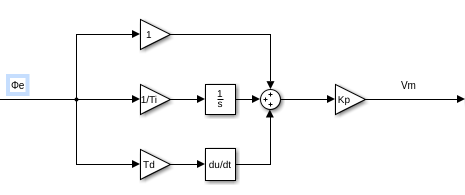
\includegraphics[scale=0.5]{figures/PID_2D.png}
  \caption[LABEL] {Block diagram of the PID controller}
\end{figure}
  
Different methods can be used to tune a PID controller as the, Zieggler-Nichols, Skogestad and Good Gain method, having in common the same goal : Get a fast response and provide a good stability. The Good Gain is the method that has been chosen as a first try to determine the parameters of the controller.\par
  
The steps of the experiment based method, the Good Gain, are the followings :\par 
 

\begin{figure}[H]
\hfill
\subfigure[Set Ti = inf , Td = 0 and Kp = 1]{
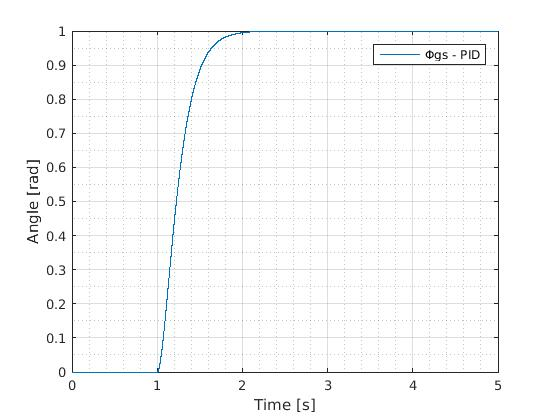
\includegraphics[scale=0.3]{figures/GG1.jpg}
\label{fig:subim11}}
\hfill
\subfigure[Increase or decrease Kp until finding a slight overshoot but a well damped response]{
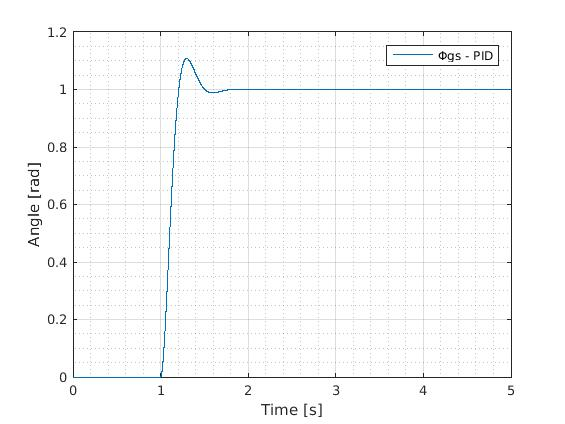
\includegraphics[scale=0.3]{figures/GG2.jpg}
\label{fig:subim12}}
\hfill
\subfigure[Set Ti = 1.5$\cdot T_{out}$]{
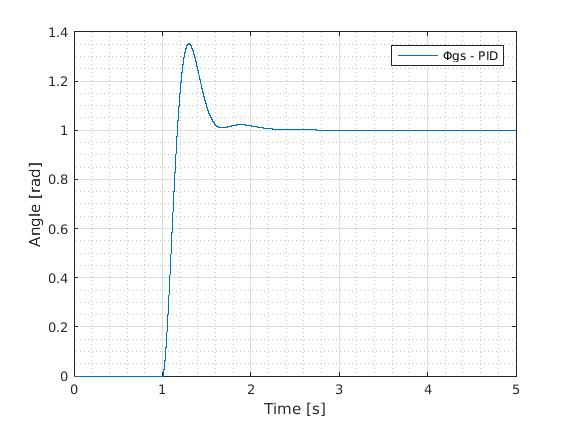
\includegraphics[scale=0.29]{figures/GG3.jpg}
\label{fig:subim12}}
\hfill
\subfigure[Set Td = $\frac{Ti}{4}$]{
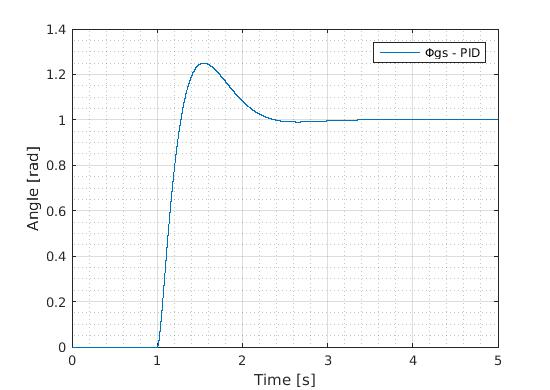
\includegraphics[scale=0.31]{figures/GG4.jpg}
\label{fig:subim12}}
\hfill
\subfigure[Final settings]{
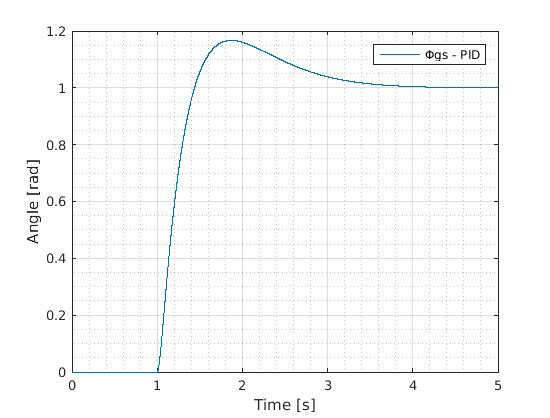
\includegraphics[scale=0.3]{figures/GG5.jpg}
\label{fig:subim12}}
\hfill

\caption{Step response for the different steps of the Good Gain method}

\end{figure}



  
\subsubsection{PID Simulink box}


\begin{figure}[H]
\centering
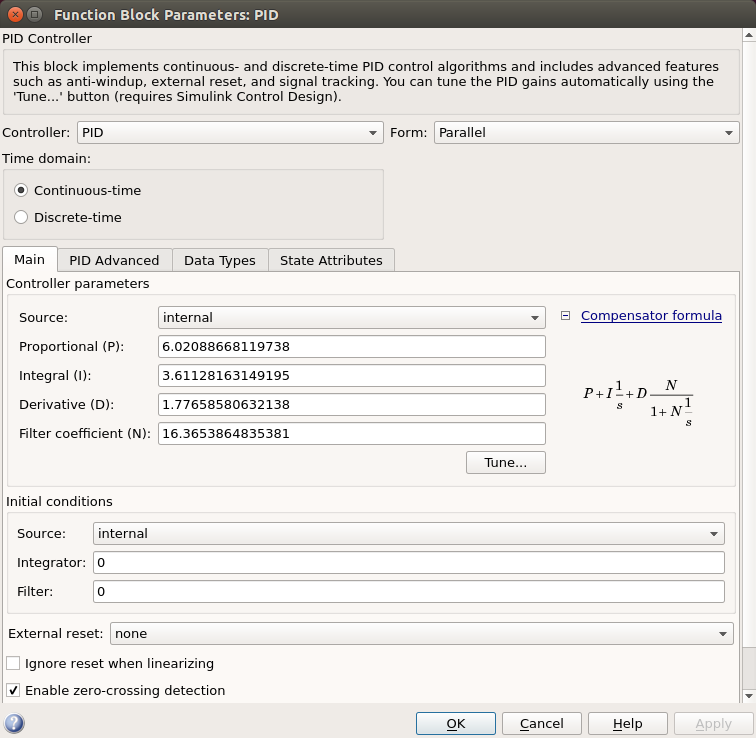
\includegraphics[scale=0.4]{figures/PID_window.png}
\caption{Inside of the PID box}
\label{dcmotor_circuit}
\end{figure}


\begin{figure}[H]
\centering
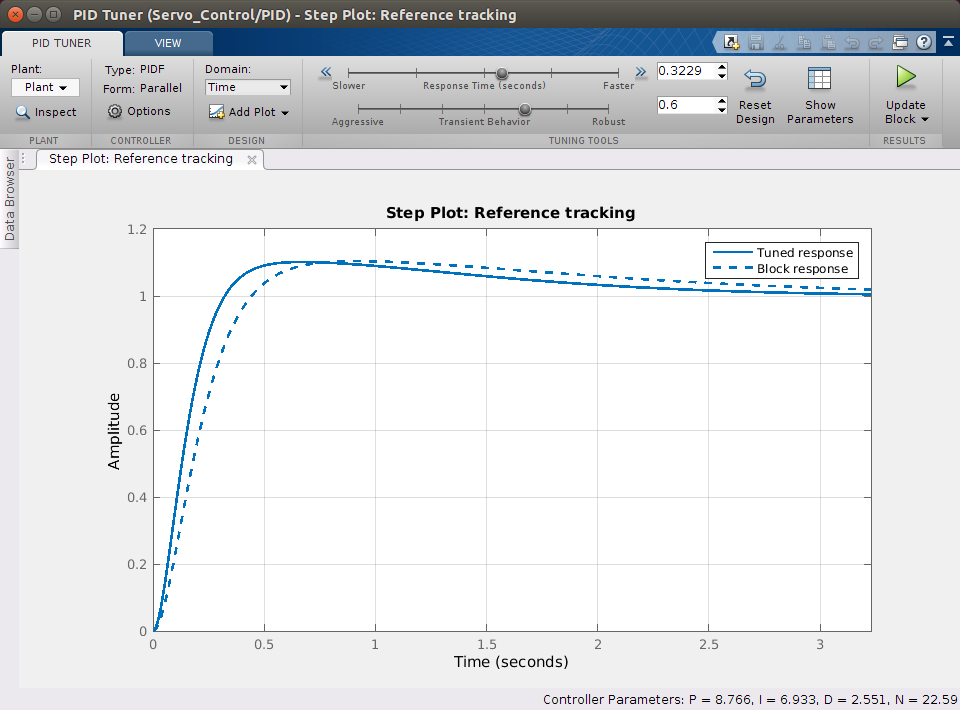
\includegraphics[scale=0.4]{figures/PID_param.png}
\caption{Tuning tool of the PID box}
\label{dcmotor_circuit}
\end{figure}
  


